\chapter{Methodology}
\label{chap:methodology}
\setlength{\parskip}{0.8em}

\section{Overall Research Design}

The research adopts a structured experimental design comprising five sequential phases: (1)~dataset selection and acquisition, (2)~data preprocessing and feature engineering, (3)~model design and training, (4)~comparative evaluation, and (5)~interpretability analysis and system design. Each phase builds on the outputs of the preceding one, and the overall pipeline is designed to be reproducible: all preprocessing parameters, model architectures, and evaluation protocols are fully specified to enable replication by independent researchers.

Figure~\ref{fig:workflow} presents the complete methodological workflow as a flowchart, illustrating the data transformation steps, decision points, and feedback loops that constitute the experimental process.

\begin{figure}[H]
\centering
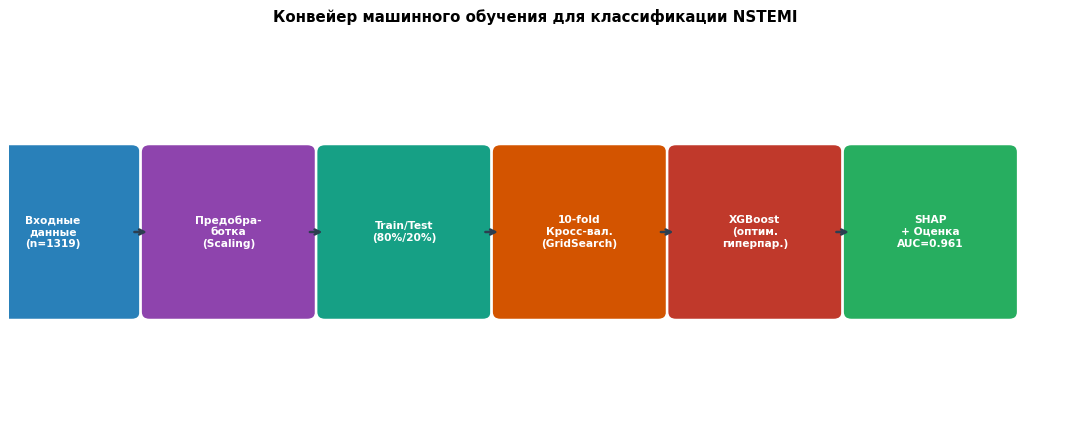
\includegraphics[width=0.92\textwidth]{figures/fig05_ml_pipeline.png}
\caption{Complete methodological workflow, from dataset selection through model training, evaluation, interpretability analysis, and system architecture design. The dashed feedback loop represents iterative hyperparameter tuning.}
\label{fig:workflow}
\end{figure}

\section{Dataset Selection and Justification}

\subsection{Selection Criteria}

The selection of the primary experimental dataset was guided by four criteria: (1)~\textbf{realism}---the dataset should reflect authentic network traffic patterns rather than purely synthetic constructs; (2)~\textbf{diversity}---the dataset should cover a broad range of contemporary attack types, including both volumetric and application-layer attacks; (3)~\textbf{richness}---the feature set should be sufficient for meaningful ML-based analysis without requiring extensive manual feature engineering; and (4)~\textbf{benchmarkability}---the dataset should be widely used in the literature to enable direct comparison with prior work.

\subsection{CICIDS2017 Dataset Description}

Based on these criteria, CICIDS2017~\cite{sharafaldin2018cicids} was selected as the primary data source. The dataset was generated over five days (3--7~July~2017) at the Canadian Institute for Cybersecurity, using CICFlowMeter to extract flow-level features from raw packet captures. It contains approximately 2.8~million flow records with 80 pre-extracted features per record.

Table~\ref{tab:attacks} summarises the attack categories present in CICIDS2017, including the tools used and the capture day.

\begin{table}[H]
\centering
\caption{Attack Categories in the CICIDS2017 Dataset}
\label{tab:attacks}
\begin{tabular}{lp{6.5cm}l}
\toprule
\textbf{Category} & \textbf{Tools / Methods Used} & \textbf{Capture Day} \\
\midrule
Benign (Normal)        & Web browsing, email, streaming, FTP, SSH         & All days  \\
DoS -- GoldenEye       & HTTP keep-alive connection flood                  & Wednesday \\
DoS -- Hulk            & HTTP GET flood with randomised URIs               & Wednesday \\
DoS -- Slowloris       & Slow HTTP header exhaustion                       & Wednesday \\
DoS -- SlowHTTPTest    & Slow read and slow POST attacks                   & Wednesday \\
DDoS LOIC              & UDP and TCP flooding                              & Friday    \\
Brute Force (FTP)      & Patator dictionary attack on FTP                  & Tuesday   \\
Brute Force (SSH)      & Hydra SSH login guessing                          & Tuesday   \\
Web -- SQL Injection   & SQLMap automated injection testing                & Thursday  \\
Web -- XSS             & BurpSuite cross-site scripting                    & Thursday  \\
Web -- Command Inj.    & Remote code execution via web forms               & Thursday  \\
Botnet (Ares)          & C\&C communication and lateral movement           & Friday    \\
Port Scan              & nmap SYN scan and service enumeration             & Friday    \\
Infiltration           & Exploitation via vulnerable applications          & Thursday  \\
\bottomrule
\end{tabular}
\end{table}

The 80 features are organised into five semantic groups:
\begin{enumerate}
    \item \textbf{Identification features:} source/destination IP address, port numbers, transport protocol (TCP/UDP/ICMP).
    \item \textbf{Connection characteristics:} session duration (Flow Duration), total packet and byte counts in each direction, forward and backward packet transfer rates.
    \item \textbf{Statistical indicators:} mean, standard deviation, minimum, and maximum of packet inter-arrival times and packet lengths in both directions.
    \item \textbf{Behavioural features:} count of connections to the same destination host/port, ratio of inbound to outbound bytes, TCP flag counts (SYN, ACK, RST, PSH).
    \item \textbf{Label:} BENIGN for normal traffic; named attack category otherwise.
\end{enumerate}

\section{Data Preprocessing Pipeline}

\subsection{Data Integration and Initial Quality Assessment}

The seven individual CSV files provided with CICIDS2017 were consolidated into a unified DataFrame using Apache Pandas. Initial inspection revealed the following data quality issues:
\begin{itemize}
    \item \textbf{Duplicate rows:} 23{,}415 exact duplicate records, arising from the CSV merging process. All duplicates were removed.
    \item \textbf{Infinite values:} Present in 12 features computed as rates or ratios in which the denominator could be zero (e.g., when Flow Duration~=~0 for instantaneous flows). Affected records were either corrected by substituting column maximum values or removed if the proportion of affected records per feature exceeded 1\%.
    \item \textbf{Missing values:} 8{,}941 records (0.32\% of total) contained NaN entries in one or more features. Given the small proportion, listwise deletion was applied without risk of significant information loss.
    \item \textbf{Label inconsistencies:} Whitespace and capitalisation inconsistencies in the class label column were standardised.
\end{itemize}

\subsection{Normalisation}

\subsubsection{Z-Score Standardisation}

All numerical features were standardised using z-score normalisation:
\begin{equation}
z_i = \frac{x_i - \mu}{\sigma}
\label{eq:zscore}
\end{equation}
where $x_i$ is the raw feature value, $\mu$ is the sample mean, and $\sigma$ is the sample standard deviation computed on the training set. This transformation ensures that all features have zero mean and unit variance, preventing features with large absolute magnitudes from disproportionately influencing distance-based and gradient-based algorithms.

\subsubsection{Logarithmic Transformation}

Network traffic features frequently exhibit heavy-tailed distributions due to the presence of large flows alongside many small ones. Features with sample skewness $\gamma_1 > 2.0$ (computed using Fisher's moment coefficient) were subjected to a log-plus-one transformation prior to z-score standardisation:
\begin{equation}
x'_i = \log(x_i + 1)
\label{eq:log_transform}
\end{equation}
The additive constant of 1 ensures that the transformation is defined for zero-valued observations. Forty-one of the 80 features met the skewness criterion and received this treatment.

\subsection{Class Imbalance Analysis and Mitigation}

\subsubsection{Imbalance Quantification}

The original CICIDS2017 dataset exhibits a pronounced class imbalance: benign traffic constitutes approximately 80.4\% of all records, while attack traffic represents 19.6\%. Within the attack class, distribution is highly heterogeneous: PortScan (158{,}930 records), DoS Hulk (231{,}073), and DDoS (128{,}027) are heavily represented, while Infiltration (36 records) and Heartbleed (11 records) are extremely rare. This imbalance, if uncorrected, would bias classifiers towards the majority class and severely impair minority-class recall.

\subsubsection{SMOTE Oversampling}

The Synthetic Minority Oversampling Technique (SMOTE) was applied to augment underrepresented attack classes. For each minority-class sample $x_i$, SMOTE generates synthetic instances by interpolating with $k$ nearest neighbours in feature space:
\begin{equation}
x_{\text{new}} = x_i + \lambda \cdot (x_{\text{nn}} - x_i), \qquad \lambda \sim \mathcal{U}(0,1)
\label{eq:smote}
\end{equation}
where $x_{\text{nn}}$ is a randomly selected neighbour from the $k$ nearest neighbours of $x_i$, and $\lambda$ is drawn from a uniform distribution. The parameter $k = 5$ was used throughout, consistent with standard practice. SMOTE was applied only to the training partition to prevent information leakage into validation or test sets.

\subsubsection{Random Undersampling}

Following SMOTE augmentation of minority classes, random undersampling of the BENIGN majority class was applied to achieve a target overall attack-to-benign ratio of approximately 1:3. This combined strategy avoids the storage and computational overhead of excessive augmentation while ensuring that the benign class remains well-represented.

\subsection{Feature Selection}

\subsubsection{Correlation Analysis}

A Pearson correlation matrix was computed for all 80 features on the preprocessed training set. Feature pairs with absolute correlation $|\rho| > 0.95$ were identified, and the member of each pair with lower predictive utility (assessed by preliminary Random Forest importance) was removed. This procedure eliminated 6 highly redundant features.

\subsubsection{Variance Inflation Factor Analysis}

The Variance Inflation Factor (VIF) was computed for all remaining features to assess multicollinearity:
\begin{equation}
\text{VIF}_j = \frac{1}{1 - R_j^2}
\label{eq:vif}
\end{equation}
where $R_j^2$ is the coefficient of determination from regressing feature $j$ on all other features. Features with $\text{VIF}_j > 10$, indicating severe multicollinearity, were excluded. This eliminated a further 4 features.

\subsubsection{Preliminary Importance Filtering}

A preliminary Random Forest with 100 trees was trained on the remaining 70 features, and features with Gini importance below $10^{-3}$ were excluded as uninformative. This removed 2 additional features. The final feature set comprises 74 attributes.

\subsection{Dataset Partitioning}

The preprocessed dataset was divided into three stratified subsets maintaining consistent class proportions:
\begin{itemize}
    \item \textbf{Training set (60\%):} Used for model fitting and cross-validation during hyperparameter optimisation.
    \item \textbf{Validation set (20\%):} Used exclusively for hyperparameter selection and early stopping decisions.
    \item \textbf{Test set (20\%):} Held out until final evaluation; never used in any training or selection decision.
\end{itemize}

Temporal ordering within each day's capture was preserved where possible to prevent information leakage.

Table~\ref{tab:preproc_stats_m} summarises the dataset statistics before and after preprocessing.

\begin{table}[H]
\centering
\caption{Dataset Statistics Before and After Preprocessing}
\label{tab:preproc_stats_m}
\begin{tabular}{lrr}
\toprule
\textbf{Property} & \textbf{Original} & \textbf{After Preprocessing} \\
\midrule
Total flow records      & 2{,}830{,}743 & 1{,}148{,}560 \\
Number of features      & 80            & 74            \\
Duplicate records       & 23{,}415      & 0             \\
Records with NaN/Inf    & 8{,}941       & 0             \\
Benign traffic (\%)     & 80.4\%        & 54.3\%        \\
Attack traffic (\%)     & 19.6\%        & 45.7\%        \\
Training samples        & ---           & 689{,}136     \\
Validation samples      & ---           & 229{,}712     \\
Test samples            & ---           & 229{,}712     \\
\bottomrule
\end{tabular}
\end{table}

\section{Machine Learning Model Design}

\subsection{Model Selection Rationale}

Six algorithms were selected to span the space from simple, highly interpretable models to complex, high-capacity models:
\begin{itemize}
    \item \textbf{Logistic Regression and KNN:} simple baselines providing performance lower bounds and feature linearity assessments.
    \item \textbf{Random Forest:} the standard ensemble baseline with built-in feature importance.
    \item \textbf{XGBoost and LightGBM:} state-of-the-art gradient boosting frameworks representing the current performance frontier for tabular data.
    \item \textbf{MLP Classifier:} a representative deep learning baseline enabling assessment of neural network performance on this task.
\end{itemize}

\subsection{Logistic Regression}

Logistic Regression models the posterior class probability via the softmax function:
\begin{equation}
P(y = k \mid x) = \frac{e^{w_k^\top x + b_k}}{\sum_{j=1}^{K} e^{w_j^\top x + b_j}}
\label{eq:softmax}
\end{equation}
where $w_k \in \mathbb{R}^d$ and $b_k \in \mathbb{R}$ are the weight vector and bias for class $k$, $K = 14$ is the number of classes, and $d = 74$ is the feature dimensionality. Parameters are estimated by minimising the multinomial cross-entropy loss with $L_2$ regularisation:
\begin{equation}
\mathcal{L} = -\frac{1}{n} \sum_{i=1}^{n} \sum_{k=1}^{K} y_{ik} \log \hat{p}_{ik} + \frac{\lambda}{2} \sum_{k=1}^{K} \|w_k\|^2
\label{eq:logloss}
\end{equation}

\subsection{K-Nearest Neighbours}

KNN classifies query point $x_q$ by majority vote among its $k$ nearest neighbours:
\begin{equation}
\hat{y} = \arg\max_{k} \sum_{i \in N_k(x_q)} \mathbb{1}[y_i = k]
\label{eq:knn}
\end{equation}
where $N_k(x_q)$ is the set of $k$ nearest neighbours of $x_q$ under Euclidean distance. $k = 5$ was selected via cross-validation.

\subsection{Random Forest}

Random Forest constructs an ensemble of $T = 200$ decision trees, each trained on a bootstrap sample $D_t$ of size $n$ with $m = \lfloor \sqrt{d} \rfloor = 8$ randomly selected features at each split:
\begin{equation}
\hat{y} = \mathrm{mode}\{h_t(x)\}_{t=1}^{T}
\label{eq:rf}
\end{equation}
Feature importance is computed as the mean decrease in Gini impurity across all trees and splits involving feature $j$:
\begin{equation}
\mathrm{Imp}_j = \frac{1}{T} \sum_{t=1}^{T} \sum_{s \in S_{tj}} \frac{n_s}{n} \left[ \mathrm{Gini}(s) - \frac{n_{s_L}}{n_s} \mathrm{Gini}(s_L) - \frac{n_{s_R}}{n_s} \mathrm{Gini}(s_R) \right]
\label{eq:gini}
\end{equation}
where $S_{tj}$ is the set of splits on feature $j$ in tree $t$, and $n_s, n_{s_L}, n_{s_R}$ are the sample counts at split node $s$ and its children.

\subsection{XGBoost}

XGBoost constructs an additive ensemble sequentially, with each new tree fitted to the negative gradient of the loss:
\begin{equation}
\hat{y}_i^{(m)} = \hat{y}_i^{(m-1)} + \eta \, f_m(x_i)
\label{eq:xgb_update}
\end{equation}
where $\eta$ is the learning rate (step shrinkage) and $f_m$ is the $m$-th tree. Each tree is fitted to minimise a second-order Taylor approximation of the regularised objective:
\begin{equation}
\mathcal{L}^{(m)} = \sum_{i=1}^{n} \left[ g_i f_m(x_i) + \tfrac{1}{2} h_i f_m(x_i)^2 \right] + \gamma T + \frac{\lambda}{2} \|w\|^2
\label{eq:xgb_obj}
\end{equation}
where $g_i = \partial_{\hat{y}} \ell(y_i, \hat{y}_i)$ and $h_i = \partial^2_{\hat{y}} \ell(y_i, \hat{y}_i)$ are the first and second gradients of the loss with respect to the prediction, $T$ is the number of leaf nodes, and $w$ are the leaf weights.

\subsection{LightGBM}

LightGBM employs a \emph{leaf-wise} (best-first) tree growth strategy, selecting at each step the leaf that maximises the reduction in loss. The split gain for a candidate split is:
\begin{equation}
\mathrm{Gain} = \frac{1}{2} \left[ \frac{G_L^2}{H_L + \lambda} + \frac{G_R^2}{H_R + \lambda} - \frac{(G_L + G_R)^2}{H_L + H_R + \lambda} \right] - \gamma
\label{eq:lgbm_gain}
\end{equation}
where $G_L = \sum_{i \in I_L} g_i$, $H_L = \sum_{i \in I_L} h_i$ are the gradient and Hessian sums for the left child, and analogously for the right child. Two additional algorithmic innovations distinguish LightGBM:
\begin{itemize}
    \item \textbf{Gradient-based One-Side Sampling (GOSS):} Retains all instances with large gradients (informative for learning) and randomly samples a fraction of small-gradient instances, reducing the training set size while preserving the effective gradient distribution.
    \item \textbf{Exclusive Feature Bundling (EFB):} Identifies groups of mutually exclusive sparse features (features that rarely take non-zero values simultaneously) and bundles them into a single composite feature, reducing effective feature dimensionality without information loss.
\end{itemize}

\subsection{MLP Classifier}

The MLP architecture is:
\begin{equation*}
x_{(74)} \xrightarrow{W_1} h_{1\,(256)} \xrightarrow{\mathrm{ReLU}} \mathrm{Drop}(0.3) \to h_{2\,(128)} \xrightarrow{\mathrm{ReLU}} \mathrm{Drop}(0.3) \to h_{3\,(64)} \xrightarrow{\mathrm{BN}} \hat{y}_{(14)}
\end{equation*}
Training minimises cross-entropy with the Adam optimiser ($\eta = 10^{-3}$, $\beta_1 = 0.9$, $\beta_2 = 0.999$), batch size 512, with early stopping at patience 10 epochs on validation F1-score.

\section{Evaluation Protocol and Metrics}

\subsection{Cross-Validation Strategy}

Hyperparameter optimisation was performed using 5-fold stratified cross-validation on the training set. For each hyperparameter configuration, the mean macro-averaged F1-score across folds was used as the optimisation criterion. The final model was retrained on the full training set using the optimal hyperparameters and evaluated once on the held-out test set.

\subsection{Performance Metrics}

Let $\mathrm{TP}, \mathrm{FP}, \mathrm{TN}, \mathrm{FN}$ denote per-class true positives, false positives, true negatives, and false negatives respectively:
\begin{align}
\mathrm{Precision}_k &= \frac{\mathrm{TP}_k}{\mathrm{TP}_k + \mathrm{FP}_k} \\
\mathrm{Recall}_k &= \frac{\mathrm{TP}_k}{\mathrm{TP}_k + \mathrm{FN}_k} \\
F_{1,k} &= 2 \cdot \frac{\mathrm{Precision}_k \cdot \mathrm{Recall}_k}{\mathrm{Precision}_k + \mathrm{Recall}_k} \\
F_1^{\text{macro}} &= \frac{1}{K} \sum_{k=1}^{K} F_{1,k} \\
\mathrm{ROC\text{-}AUC} &= \int_{0}^{1} \mathrm{TPR}(t)\, d\,\mathrm{FPR}(t)
\end{align}
Macro-averaging was selected over weighted or micro-averaging because it weights all classes equally, ensuring that rare attack categories (e.g., Infiltration, Heartbleed) receive the same contribution to the aggregate metric as common ones. This choice is consistent with the security objective: missing a rare attack type is as operationally serious as misclassifying a common one.

\subsection{Interpretability Methods}

\subsubsection{SHAP}

SHAP assigns each feature $j$ a Shapley value $\phi_j$ representing its average marginal contribution to the model output across all possible feature subsets~\cite{shone2018deep}:
\begin{equation}
\phi_j = \sum_{S \subseteq F \setminus \{j\}} \frac{|S|! \, (|F| - |S| - 1)!}{|F|!} \left[ f_{S \cup \{j\}}(x) - f_S(x) \right]
\label{eq:shap}
\end{equation}
For tree-based models, SHAP values can be computed exactly in polynomial time using TreeExplainer~\cite{shone2018deep}, making it tractable for large ensembles such as LightGBM.

\subsubsection{LIME}

LIME approximates the model $f$ locally around a query instance $x$ with an interpretable linear model $g$ by minimising:
\begin{equation}
\xi(x) = \arg\min_{g \in G} \, \mathcal{L}(f, g, \pi_x) + \Omega(g)
\label{eq:lime}
\end{equation}
where $\pi_x(z) = \exp(-D(x, z)^2 / \sigma^2)$ is an exponential kernel weighting sampled points by proximity to $x$, and $\Omega(g)$ penalises the complexity (number of non-zero coefficients) of $g$. The locally linear model coefficients provide feature-level explanations specific to the individual prediction.
